% Figure s05f04_topology (Session 5): same gap, different topology, seen from above.
% The image is rendered by figures/blender/s05f04_topology.py; the coordinates of the labels come from
% figures/blender/out/s05f04_topology_anchors.tex. Build with figures/blender/build_figure.sh s05f04_topology.
\documentclass[11pt,tikz,border=0pt]{standalone}
\usepackage[T1]{fontenc}
\usepackage{amsmath,amssymb,graphicx,bm}
\usepackage{xcolor}
\usetikzlibrary{arrows.meta,calc}
% The three label colors of the figures, with the same values as in src/figures_preamble.tex.
\definecolor{aqmaccent}{RGB}{31,78,121}
\definecolor{aqmbroken}{RGB}{168,42,34}
\definecolor{aqmmuted}{RGB}{125,125,125}

% Shared TikZ styles of the overlays: axis arrows drawn on top of the renders, between anchors
% written by the scripts, so that they can be adjusted without rendering again.
\tikzset{
  axarrow/.style={line width=0.6pt, draw=black!70, -{Stealth[length=4.5pt,width=3.5pt]}},
  axlbl/.style={font=\small, inner sep=1.5pt},
}
% A discrete color key: \aqmkey{(x,y)}{color 1}{label 1}{color 2}{label 2} draws two swatches in a
% column with their labels, anchored at its north west corner. The colors are the sRGB values
% used in the render, defined below.
\definecolor{keypos}{RGB}{118,158,198}
\definecolor{keyneg}{RGB}{214,150,132}
\definecolor{keyup}{RGB}{224,62,40}
\definecolor{keydown}{RGB}{40,92,200}
\definecolor{keydark}{RGB}{31,78,121}
\definecolor{keylight}{RGB}{118,158,198}
\newcommand{\aqmkey}[5]{%
  \begin{scope}[shift={#1}]
    \fill[#2, draw=black!40, line width=0.3pt] (0,-0.32) rectangle (0.32,0);
    \node[font=\small, anchor=west, inner sep=1.5pt] at (0.38,-0.16) {#3};
    \fill[#4, draw=black!40, line width=0.3pt] (0,-0.74) rectangle (0.32,-0.42);
    \node[font=\small, anchor=west, inner sep=1.5pt] at (0.38,-0.58) {#5};
  \end{scope}}
% The same key in one row, for a figure with no room for a column.
\newcommand{\aqmkeyrow}[5]{%
  \begin{scope}[shift={#1}]
    \fill[#2, draw=black!40, line width=0.3pt] (0,-0.32) rectangle (0.32,0);
    \node[font=\small, anchor=west, inner sep=1.5pt] (k1) at (0.38,-0.16) {#3};
    \fill[#4, draw=black!40, line width=0.3pt] ([xshift=0.25cm]k1.east |- 0,-0.32) rectangle ++(0.32,0.32);
    \node[font=\small, anchor=west, inner sep=1.5pt] at ([xshift=0.63cm]k1.east) {#5};
  \end{scope}}

\newlength{\figw}\setlength{\figw}{12.5cm}   % 0.8 of the text width

\begin{document}
\begin{tikzpicture}[lbl/.style={font=\small, inner sep=1.5pt}, pnl/.style={font=\small\bfseries, inner sep=1.5pt}]
  \node[anchor=south west, inner sep=0pt] at (0,0)
    {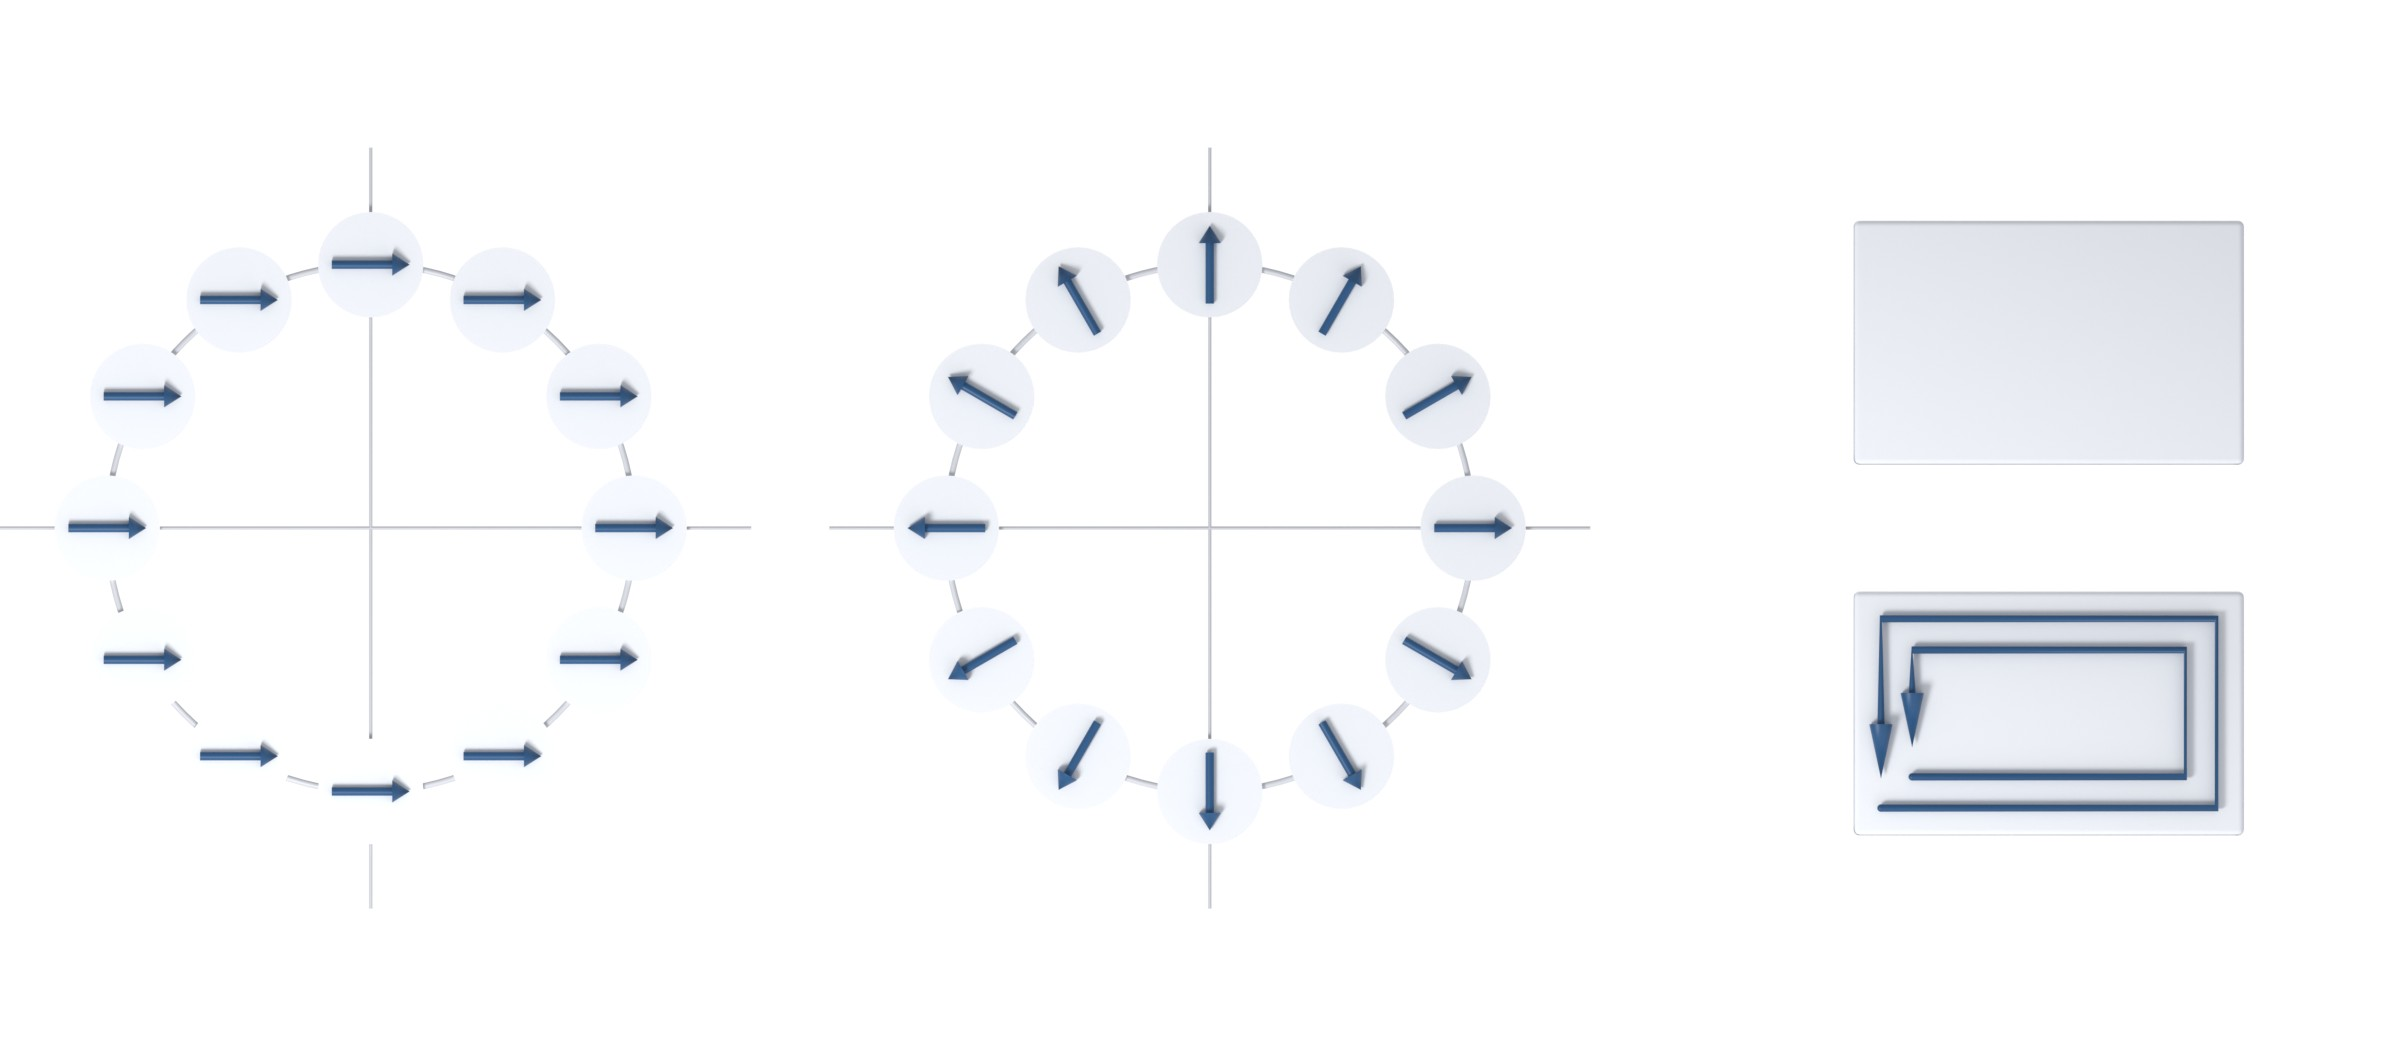
\includegraphics[width=\figw]{../blender/out/s05f04_topology.jpg}};
  %% written by figlib.py; x and y in units of the image width
\coordinate (apanel) at (0.0163\figw,0.3828\figw);
\coordinate (abelow) at (0.1545\figw,0.0494\figw);
\coordinate (bpanel) at (0.3659\figw,0.3828\figw);
\coordinate (bbelow) at (0.5041\figw,0.0494\figw);
\coordinate (ctriv) at (0.8537\figw,0.2344\figw);
\coordinate (cchir) at (0.8537\figw,0.0799\figw);
\coordinate (cpanel) at (0.7561\figw,0.3828\figw);

  \node[lbl, anchor=south west] at (apanel) {\textbf{(a)}\quad $s$-wave};
  \node[lbl, anchor=south west] at (bpanel) {\textbf{(b)}\quad chiral $p$-wave};
  \node[lbl, anchor=south west] at (cpanel) {\textbf{(c)}};
  \node[lbl, anchor=north] at (abelow) {winding $0$, $C=0$};
  \node[lbl, anchor=north] at (bbelow) {winding $1$};
  \node[lbl, anchor=north, text=aqmmuted] at (ctriv) {trivial};
  \node[lbl, anchor=north, text=aqmaccent] at (cchir) {chiral, $C=2$};
  \node[axlbl, anchor=north east] at (akx) {$k_x$};
  \node[axlbl, anchor=south west] at (aky) {$k_y$};
  \node[axlbl, anchor=north east] at (bkx) {$k_x$};
  \node[axlbl, anchor=south west] at (bky) {$k_y$};
\end{tikzpicture}
\end{document}
